\documentclass[tikz]{standalone}
\usepackage{tikz} 
\usepackage{pgfplots}
\pgfplotsset{compat=newest, ticks=none}
\usetikzlibrary{calc}

\definecolor{redp}{rgb}{0.78, 0.03, 0.08}
\definecolor{greenp}{rgb}{0.0, 0.51, 0.5}
\definecolor{yellowp}{rgb}{0.59, 0.44, 0.09}

\begin{document}
	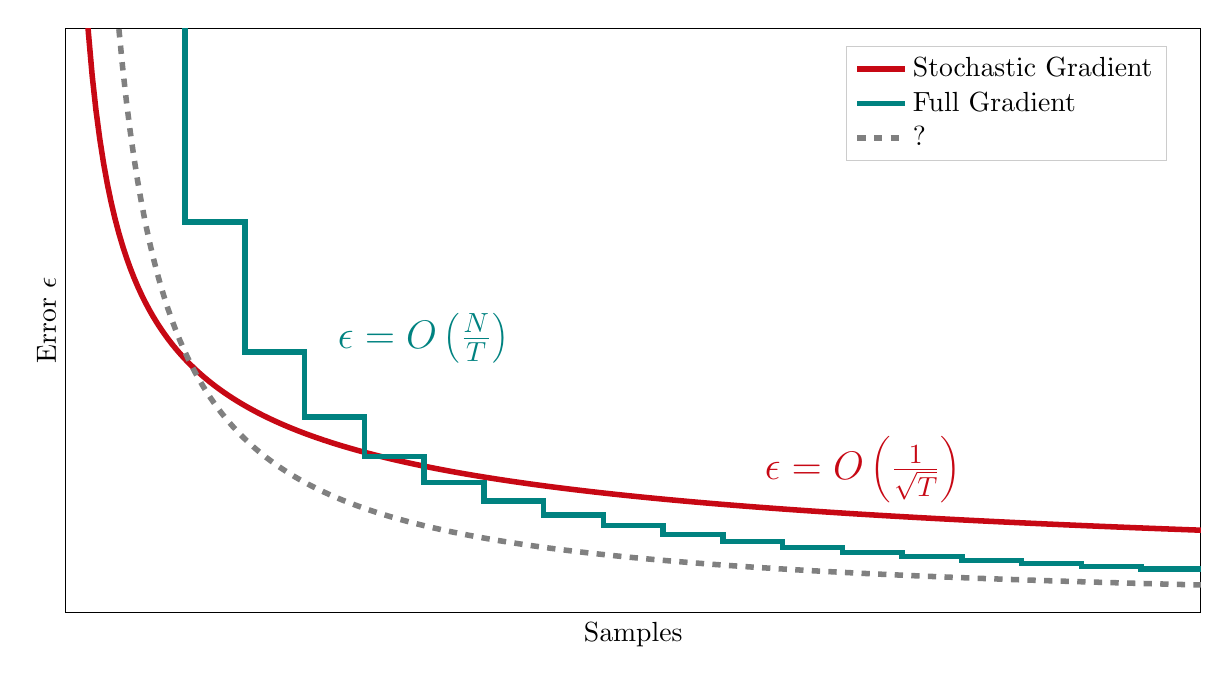
\begin{tikzpicture}
	\begin{axis}[
		width=16cm, height=9cm,
		xlabel={Samples},
		ylabel={Error $\epsilon$},
		xmin=0, xmax=16,
		ymin=0, ymax=16,
		x grid style={lightgray!92.02614379084967!black},
		y grid style={lightgray!92.02614379084967!black},
		legend cell align={left},
		legend entries={{Stochastic Gradient},{Full Gradient},{?}},
		legend style={at={(0.97,0.97)}, anchor=north east, draw=white!80.0!black},
		]
		\addplot
		[line width=2pt,
		redp,
		domain
		=0:16,
		samples
		=300,
		]
		{9/sqrt(x)}
		node[above,pos=.9] {\Large{\textbf{$\epsilon=O\left(\frac{1}{\sqrt{T}}\right)$}}};
		%
		\addplot
		[line width=2pt,
		const plot,
		greenp,
		domain
		=0:16,
		samples
		=20,
		]
		{18/(x)}
		node[above,pos=.5, xshift=2cm] {\Large{\textbf{$\epsilon=O\left(\frac{N}{T}\right)$}}};
		%
		\addplot
		[line width=2pt,
		gray,
		dashed,
		domain
		=0:16,
		samples
		=300,
		]
		{12/(x)};
	\end{axis}
	\end{tikzpicture}
\end{document}